\documentclass{beamer}
\usepackage{graphicx}
\usepackage{amsmath}

\title{Detailed Explanations of Monetary Policy Concepts}
\author{Charles Ancel}
\date{July 15, 2024}

\begin{document}

\frame{\titlepage}

\section{Federal Reserve's Process for Implementing Monetary Policy}

\begin{frame}
    \frametitle{Main Instrument of the Fed's Monetary Policy}
    \begin{itemize}
        \item \textbf{Federal Funds Rate:} The interest rate at which banks lend reserves to each other overnight.
        \item \textbf{Open Market Operations:} Used to influence the federal funds rate.
    \end{itemize}
\end{frame}

\begin{frame}
    \frametitle{Decision Process in FOMC Meetings and Public Announcement}
    \begin{itemize}
        \item \textbf{FOMC Meetings:} Review economic data, consider forecasts, and vote on the appropriate federal funds rate.
        \item \textbf{Public Announcement:} Decisions announced via press releases and the Fed's website. The Fed Chair holds a press conference to explain the rationale behind decisions.
    \end{itemize}
\end{frame}

\begin{frame}
    \frametitle{Implementation by the New York Fed}
    \begin{itemize}
        \item \textbf{Open Market Trading Desk:} Conducts operations to influence the supply of reserves.
    \end{itemize}
\end{frame}

\section{Objectives of Monetary Policy}

\begin{frame}
    \frametitle{Main Objectives and Loss Function}
    \begin{itemize}
        \item \textbf{Price Stability:} Keeping inflation low and stable.
        \item \textbf{Full Employment:} Achieving the highest level of employment.
        \item \textbf{Loss Function:}
        \begin{equation*}
            L = \lambda {(\pi_t - \pi^*)}^2 + {(y_t - y^*)}^2
        \end{equation*}
        where \(\pi_t\) is the inflation rate, \(\pi^*\) is the target inflation rate, \(y_t\) is the output, and \(y^*\) is the potential output.
    \end{itemize}
\end{frame}

\section{Term Structure of Interest Rates}

\begin{frame}
    \frametitle{Term Structure of Interest Rates}
    \begin{itemize}
        \item \textbf{Concept:} Represents the relationship between interest rates of bonds with different maturities.
        \item \textbf{Relevance to Monetary Policy:} Short-term rates set by the Fed affect longer-term rates, achieving policy objectives.
    \end{itemize}
\end{frame}

\begin{frame}
    \frametitle{Graph: Term Structure of Interest Rates}
    \begin{center}
        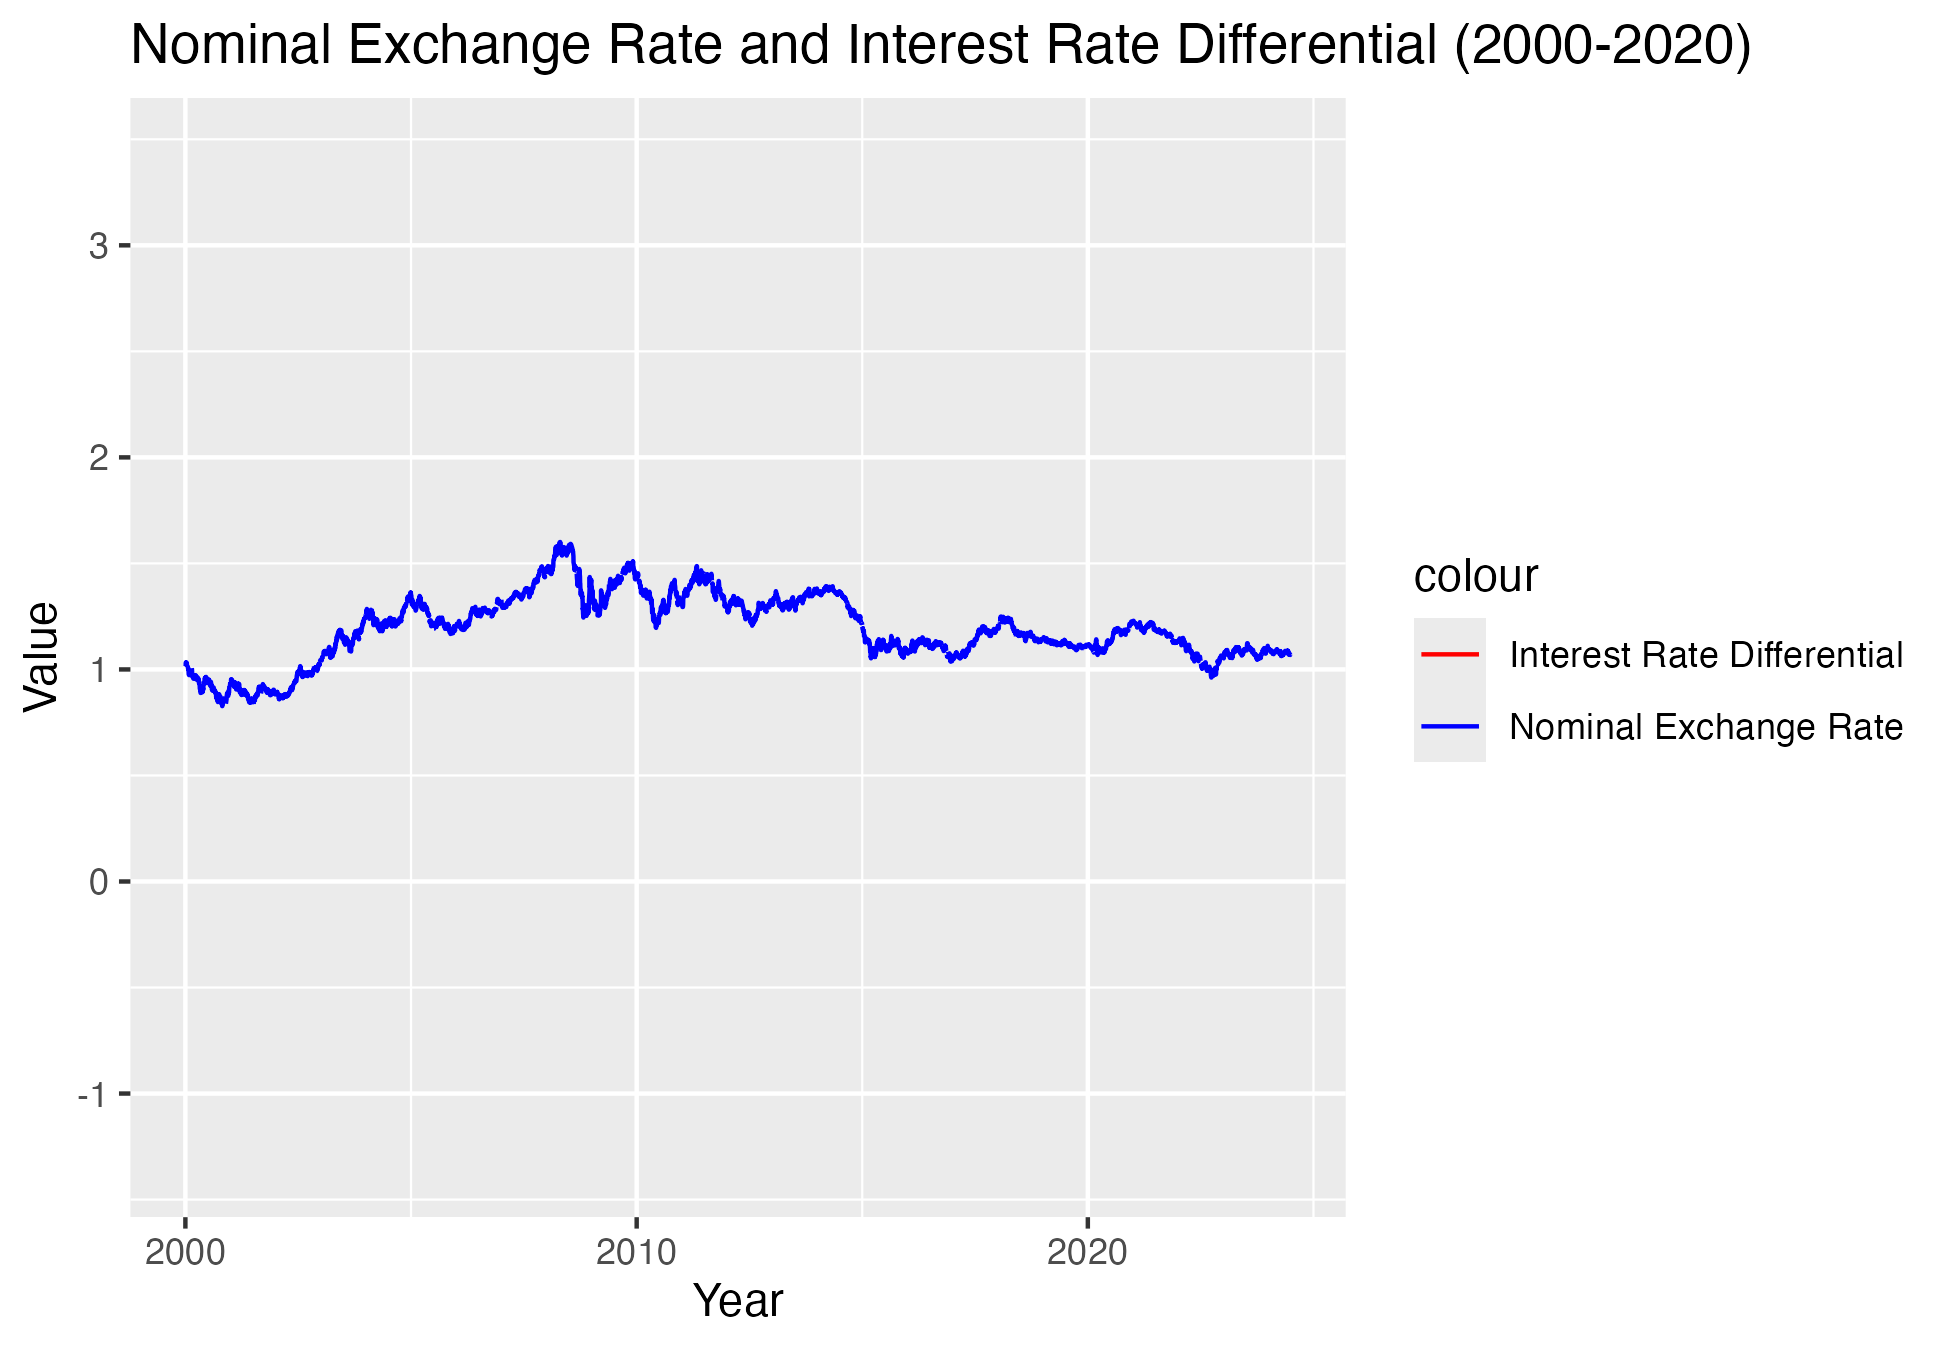
\includegraphics[width=0.8\textwidth]{/Users/cancel/Personal/Coursework/Econ425/VA2/R/Nominal_Exchange_Rate_and_Interest_Rate_Differential.png}
    \end{center}
\end{frame}

\section{MP Curve and Optimal Monetary Policy}

\begin{frame}
    \frametitle{MP Curve: Optimal and Non-Optimal Conditions}
    \begin{itemize}
        \item \textbf{MP Curve:} Shows the relationship between the real interest rate and inflation.
        \item \textbf{Non-Optimal Conditions:} May not be optimal if it doesn't account for other economic conditions or shocks.
    \end{itemize}
\end{frame}

\begin{frame}
    \frametitle{Graph: MP Curve}
    \begin{center}
        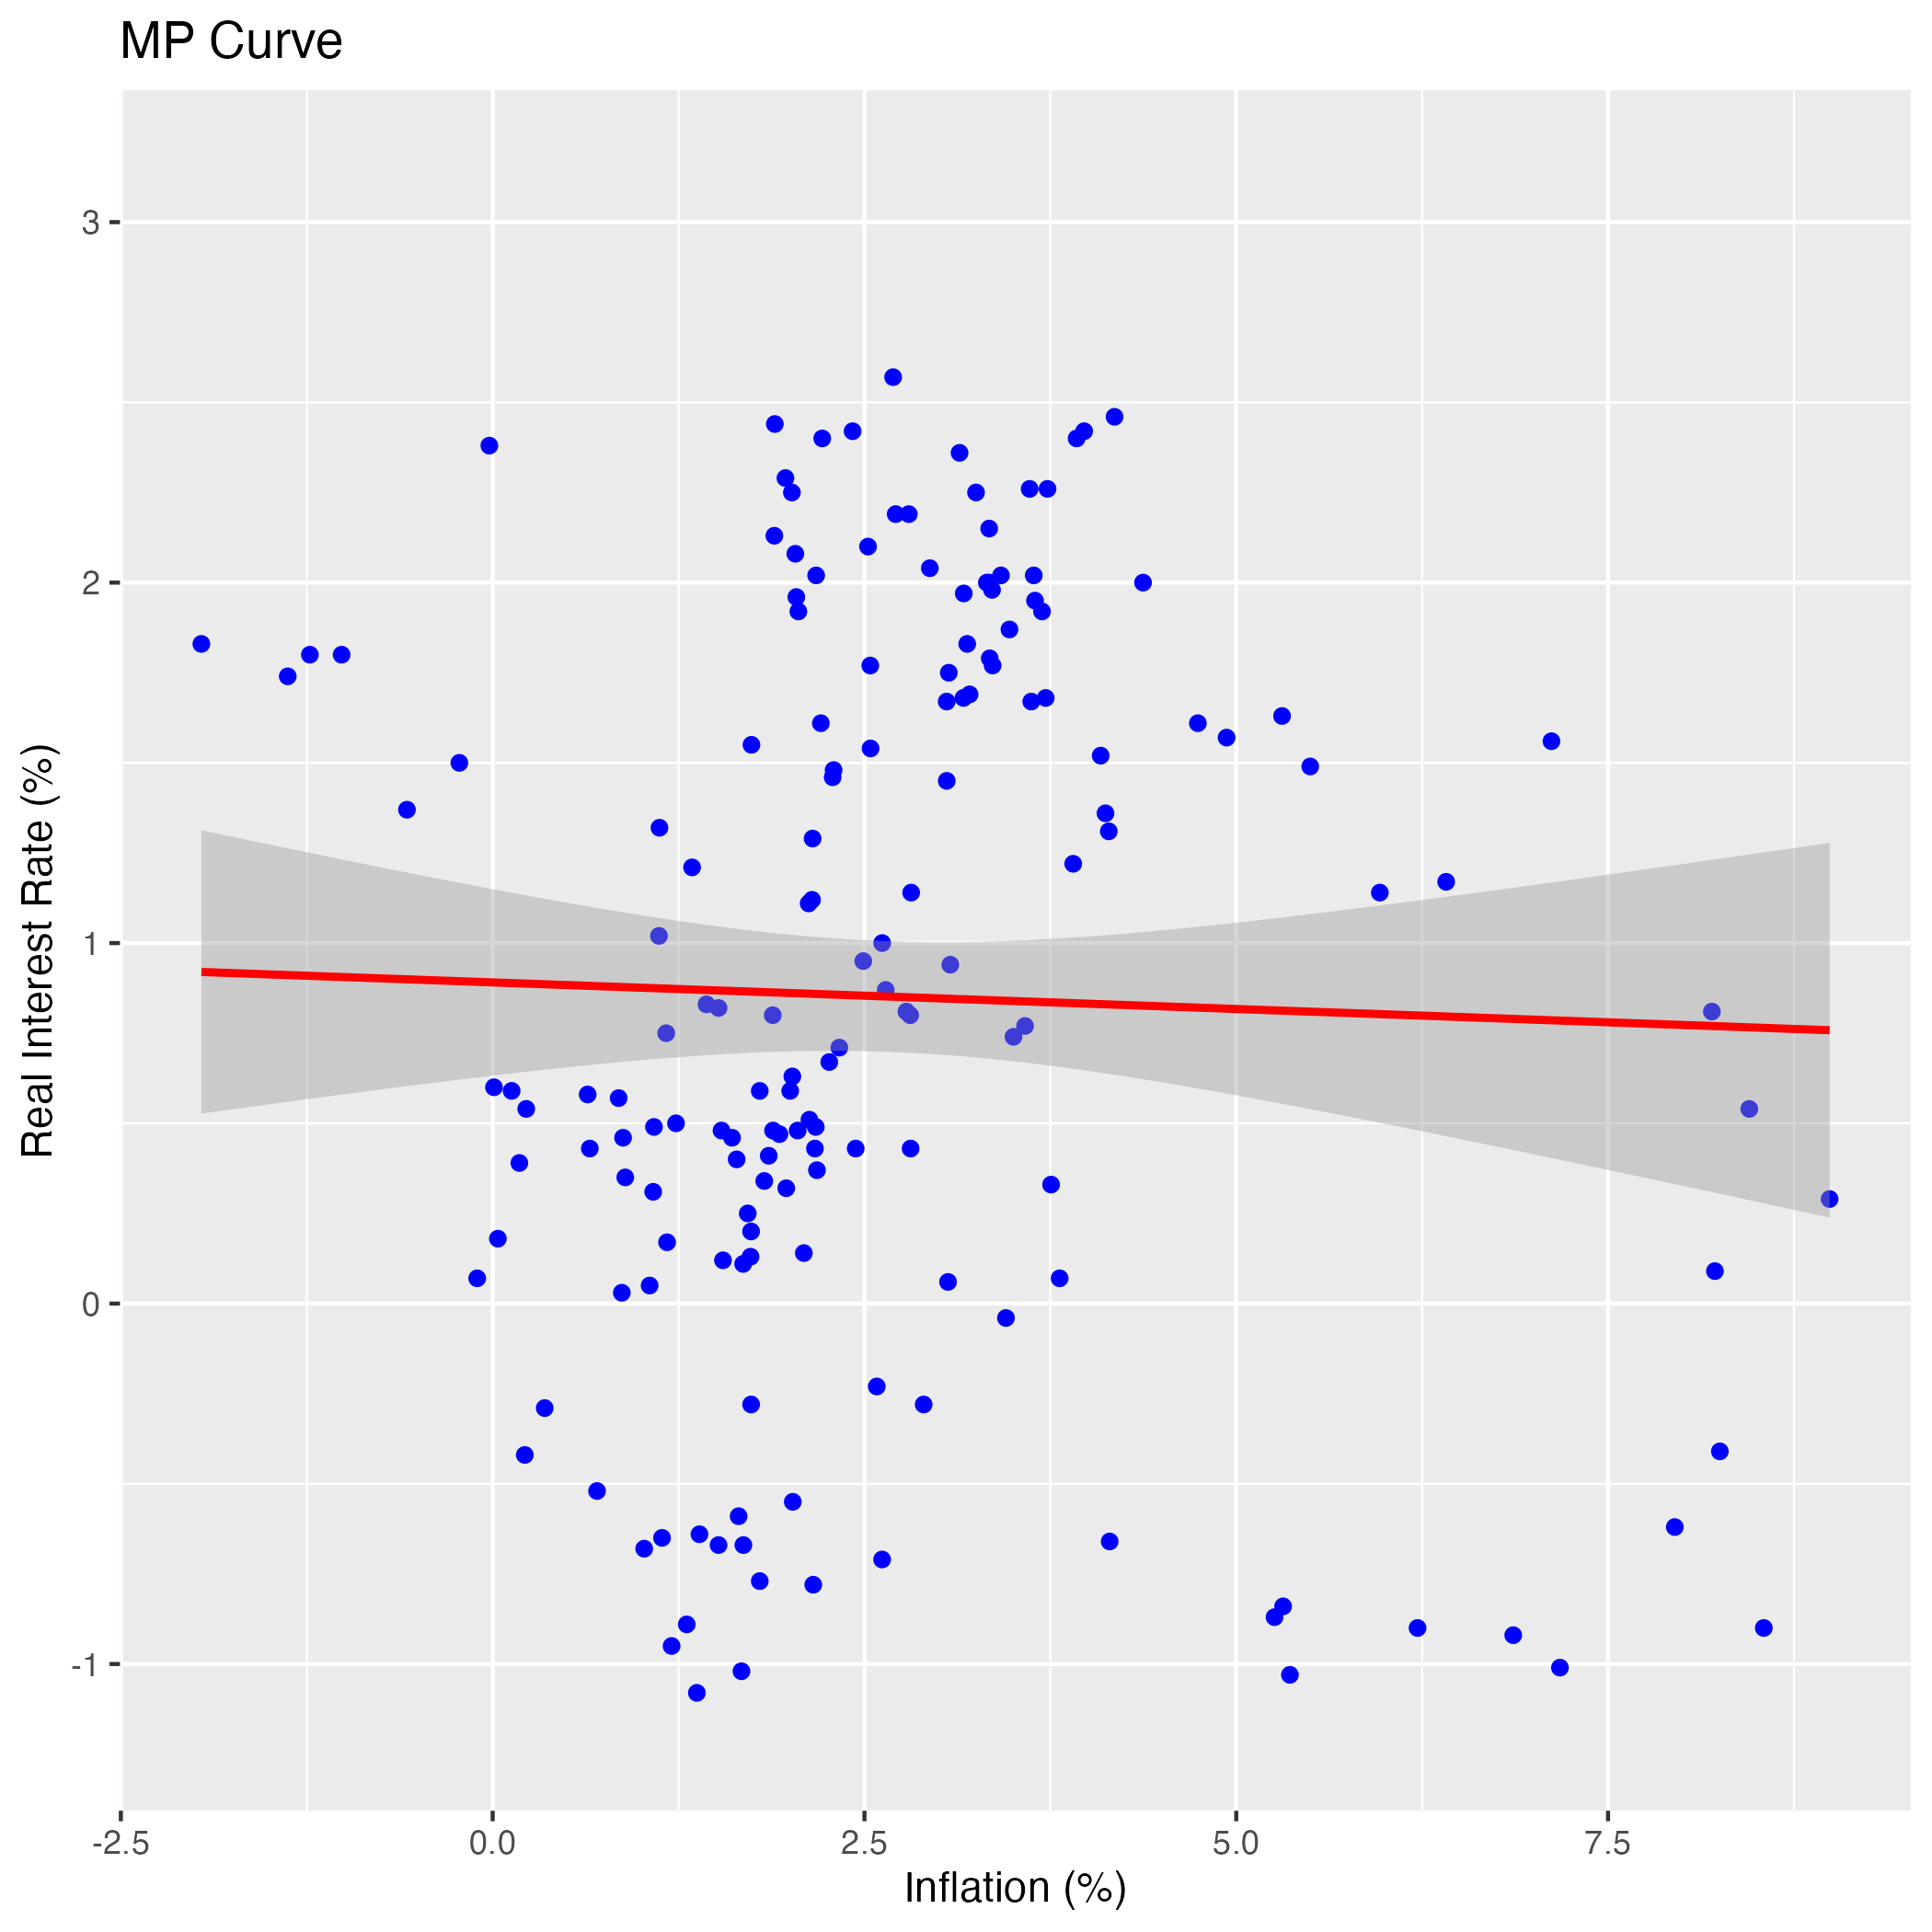
\includegraphics[width=0.8\textwidth]{/Users/cancel/Personal/Coursework/Econ425/VA2/R/MP_Curve.png}
    \end{center}
\end{frame}

\section{The Taylor Rule}

\begin{frame}
    \frametitle{The Taylor Rule}
    \begin{itemize}
        \item \textbf{Definition and Formula:}
        \begin{equation*}
            i_t = r^* + \pi_t + 0.5(\pi_t - \pi^*) + 0.5(y_t - y^*)
        \end{equation*}
        \item \textbf{Optimality and Usefulness:} Useful for its simplicity and transparency.
    \end{itemize}
\end{frame}

\section{Dangers of Not Following the Taylor Principle}

\begin{frame}
    \frametitle{Taylor Principle and Its Consequences}
    \begin{itemize}
        \item \textbf{Taylor Principle:} Central bank should raise nominal interest rates by more than the increase in inflation.
        \item \textbf{Consequences of Ignoring:} Failing to follow can lead to runaway inflation.
    \end{itemize}
\end{frame}

\begin{frame}
    \frametitle{Graph: Taylor Principle}
    \begin{center}
        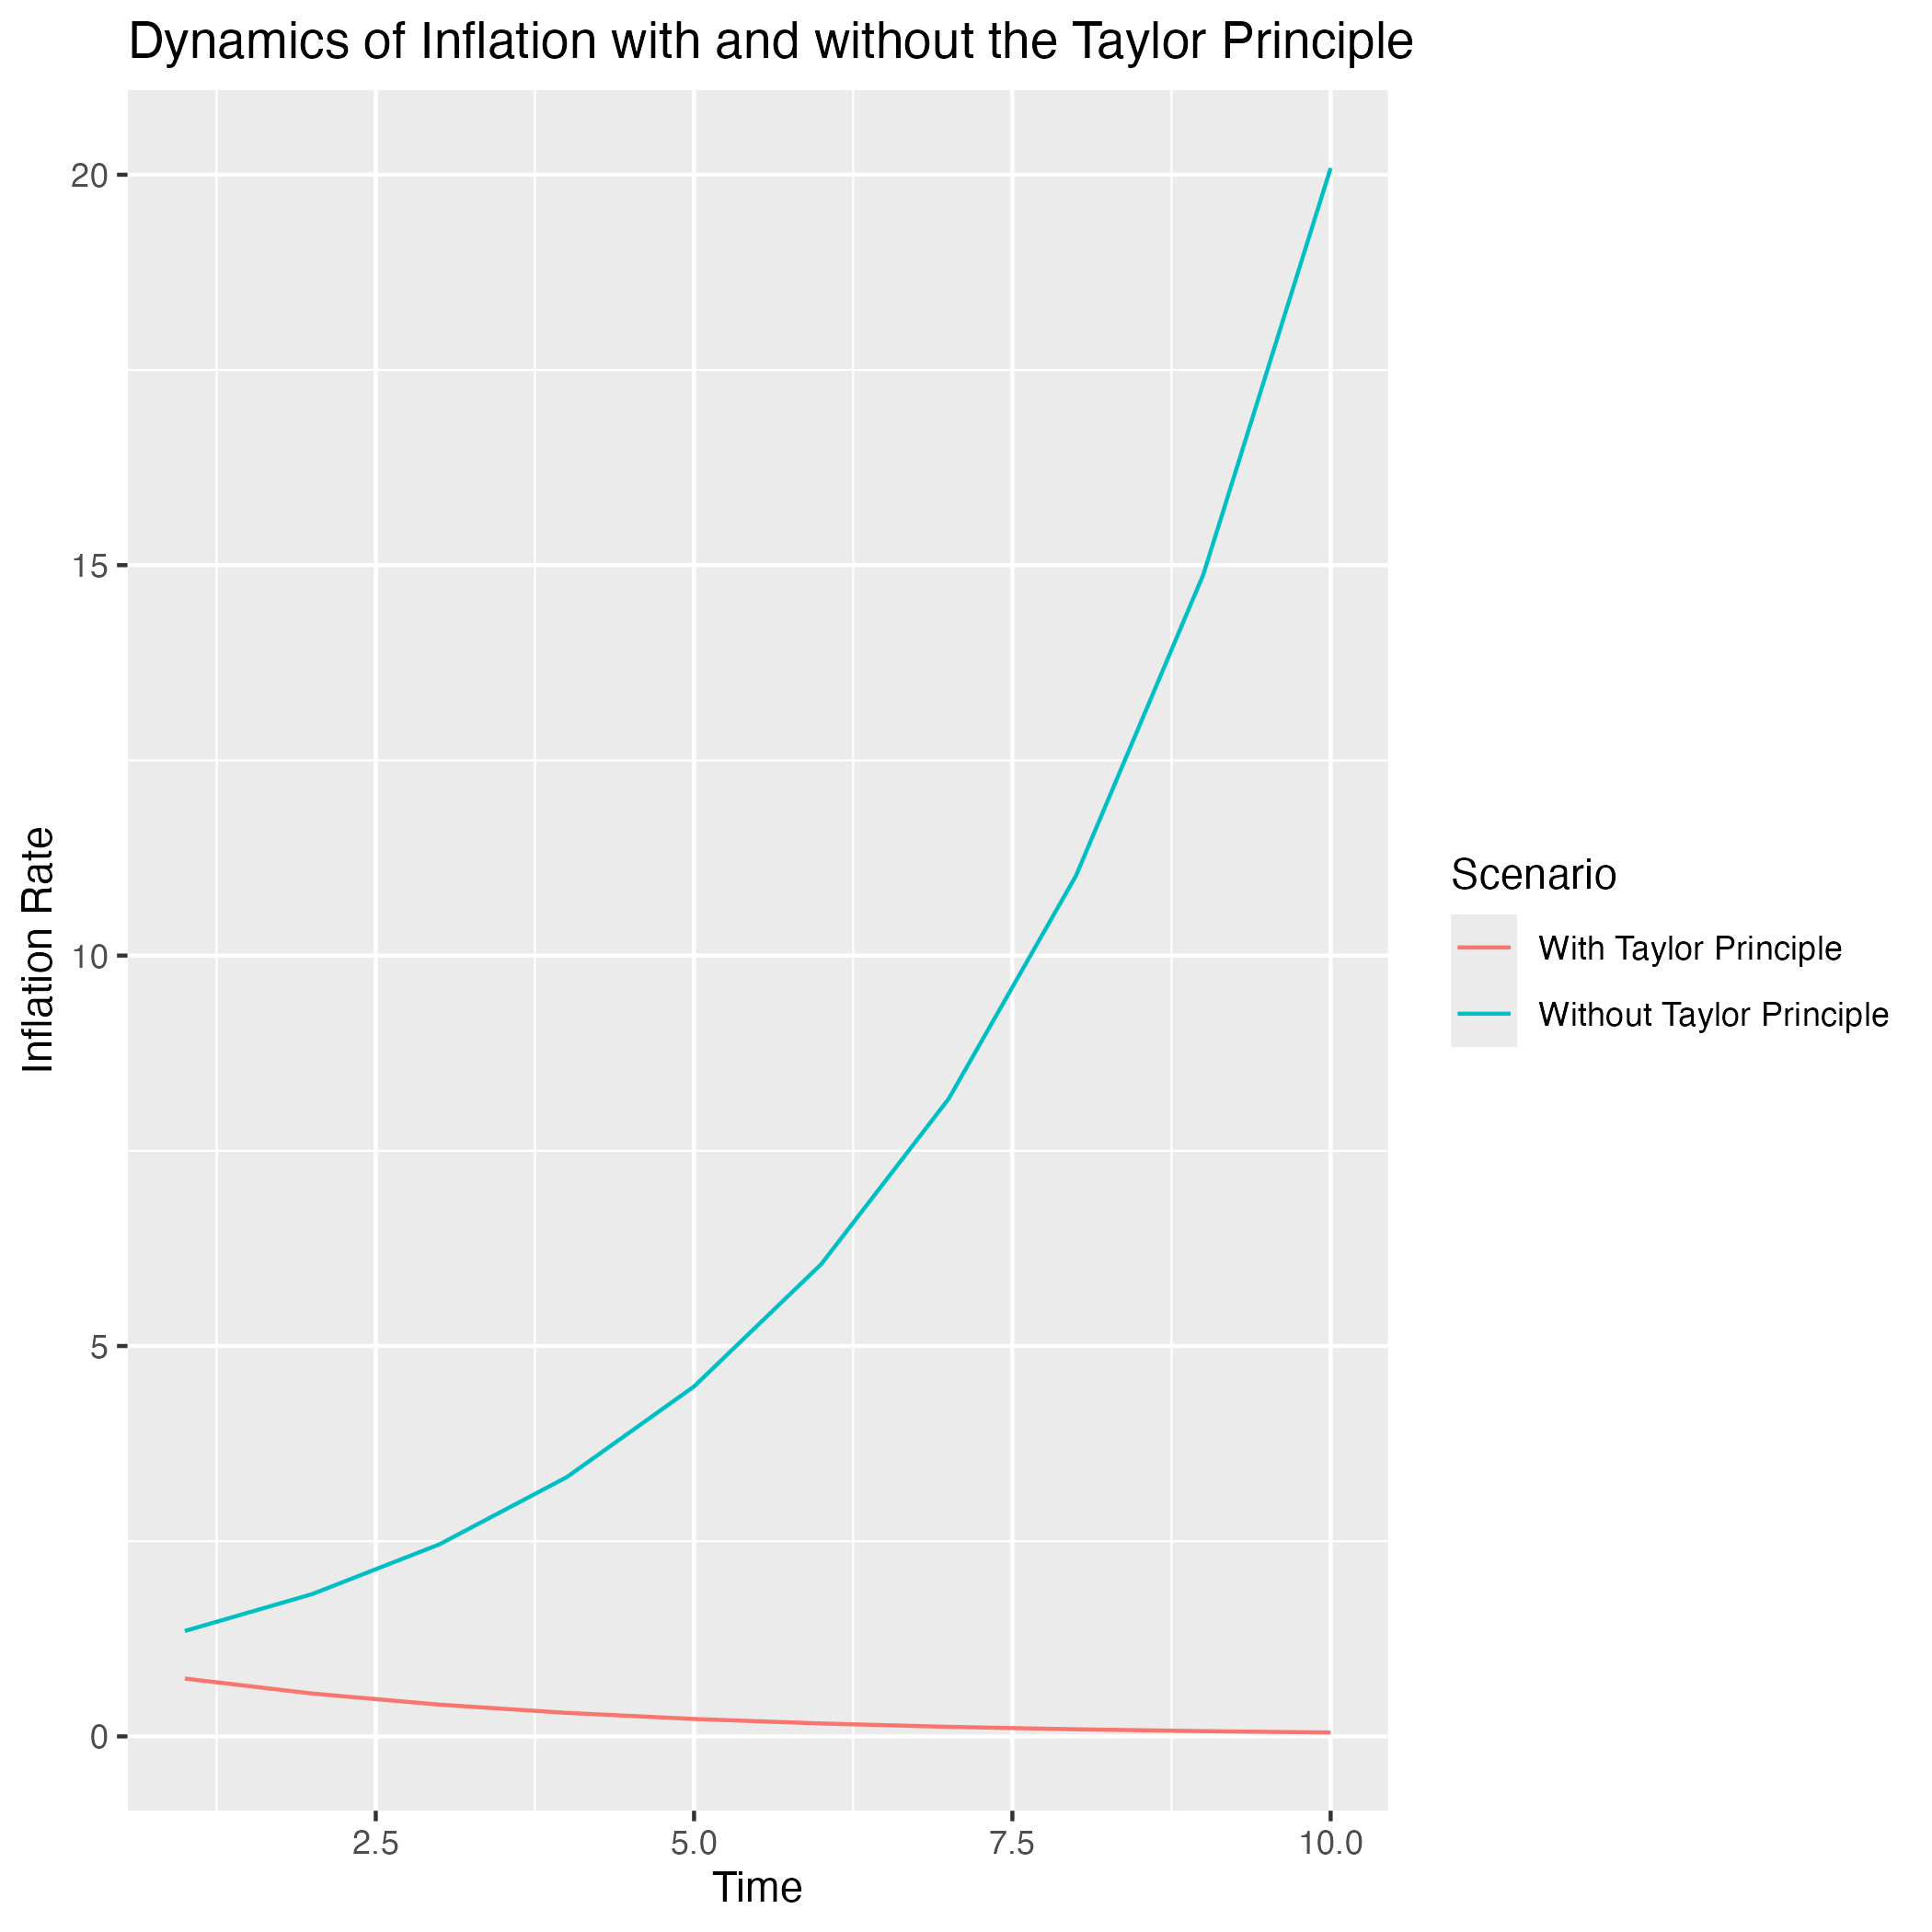
\includegraphics[width=0.8\textwidth]{/Users/cancel/Personal/Coursework/Econ425/VA2/R/InflationDynamics.png}
    \end{center}
\end{frame}

\section{Optimal Stabilization vs. Optimal Disinflation}

\begin{frame}
    \frametitle{Optimal Stabilization and Disinflation}
    \begin{itemize}
        \item \textbf{Optimal Stabilization:} Aims to minimize variance of inflation and output.
        \item \textbf{Optimal Disinflation:} Reducing inflation to a lower target with minimal output loss.
    \end{itemize}
\end{frame}

\section{Importance of Expectations in Macroeconomics}

\begin{frame}
    \frametitle{Expectations in Macroeconomics}
    \begin{itemize}
        \item \textbf{Role of Expectations:} Influence current behavior.
        \item \textbf{Rational Expectations:} Models assume rational expectations for accurate predictions.
    \end{itemize}
\end{frame}

\section{The Lucas Critique}

\begin{frame}
    \frametitle{The Lucas Critique}
    \begin{itemize}
        \item \textbf{Explanation:} Traditional models fail to account for changes in policy regimes.
        \item \textbf{Importance for Policy Making:} Need for models that incorporate rational expectations and policy impacts on behavior.
    \end{itemize}
\end{frame}

\section{Central Bank Preferences and Policy}

\begin{frame}
    \frametitle{Central Bank Preferences and Policy}
    \begin{itemize}
        \item \textbf{Dangers of Alignment:} Too aligned with public preferences can lead to inflationary policies.
        \item \textbf{Solution: Central Bank Independence:} Mitigates risks, balancing long-term stability with short-term flexibility.
    \end{itemize}
\end{frame}

\section{Conclusion}

\begin{frame}
    \frametitle{Conclusion}
    \begin{itemize}
        \item Thank you for your attention. This concludes my discussion on monetary policy concepts. If you have any questions, please feel free to ask.
    \end{itemize}
\end{frame}

\end{document}
